\documentclass[12pt]{article}

% TEMPLATE DEFAULT PACKAGES
\usepackage{amssymb,amsmath,amsfonts,eurosym,geometry,ulem,graphicx,color,setspace,sectsty,comment,natbib,pdflscape,array,adjustbox}

% ADDED PACKAGES FOR THIS MANUSCRIPT
\usepackage{palatino,newtxmath,multirow,titlesec,threeparttable,tabu,booktabs,titlesec,threeparttable,mathtools,bm,bbm,subcaption,pdflscape,tcolorbox,mathrsfs}
% endfloat,

\usepackage{afterpage}
\usepackage[hyphens]{url}
\usepackage[margin=1cm]{caption}

\usepackage[draft]{hyperref}
\newcommand{\tim}{$\,\times\,$}
% FIGURES & TABLES CAPTION STYLING
\captionsetup[figure]{labelfont={bf},name={Figure},labelsep=period}
\captionsetup[table]{labelfont={bf},name={Table},labelsep=period}

% SECTION TITLE SETTINGS
\titlelabel{\thetitle.\enskip}
\titleformat*{\section}{\large\bfseries}
\titleformat*{\subsection}{\normalsize\bfseries}

% COLUMN TYPES
\newcolumntype{L}[1]{>{\raggedright\let\newline\\\arraybackslash\hspace{0pt}}m{#1}}
\newcolumntype{C}{>{\centering\arraybackslash}p{5.2em}}
\newcolumntype{D}{>{\centering\arraybackslash}p{5em}}
\newcolumntype{R}[1]{>{\raggedleft\let\newline\\\arraybackslash\hspace{0pt}}m{#1}}


% MARGINS AND SPACING
\normalem
\geometry{left=1.1in,right=1.1in,top=1.0in,bottom=1.0in}
\setlength{\parskip}{2.5pt}

% SPECIAL CELL 
\newcommand{\specialcell}[2][c]{%
	\begin{tabular}[#1]{@{}l@{}}#2\end{tabular}}

% NO INDENT ON FOOTNOTES
\usepackage[hang,flushmargin]{footmisc}

\begin{document}

\Large New Method 2
% \begin{figure}[t]
% \caption{Transaction Price Histogram}\label{figure:transactionhist}
% \centering
% \tcbox[colback=white,boxrule=.35mm,boxsep=0mm]{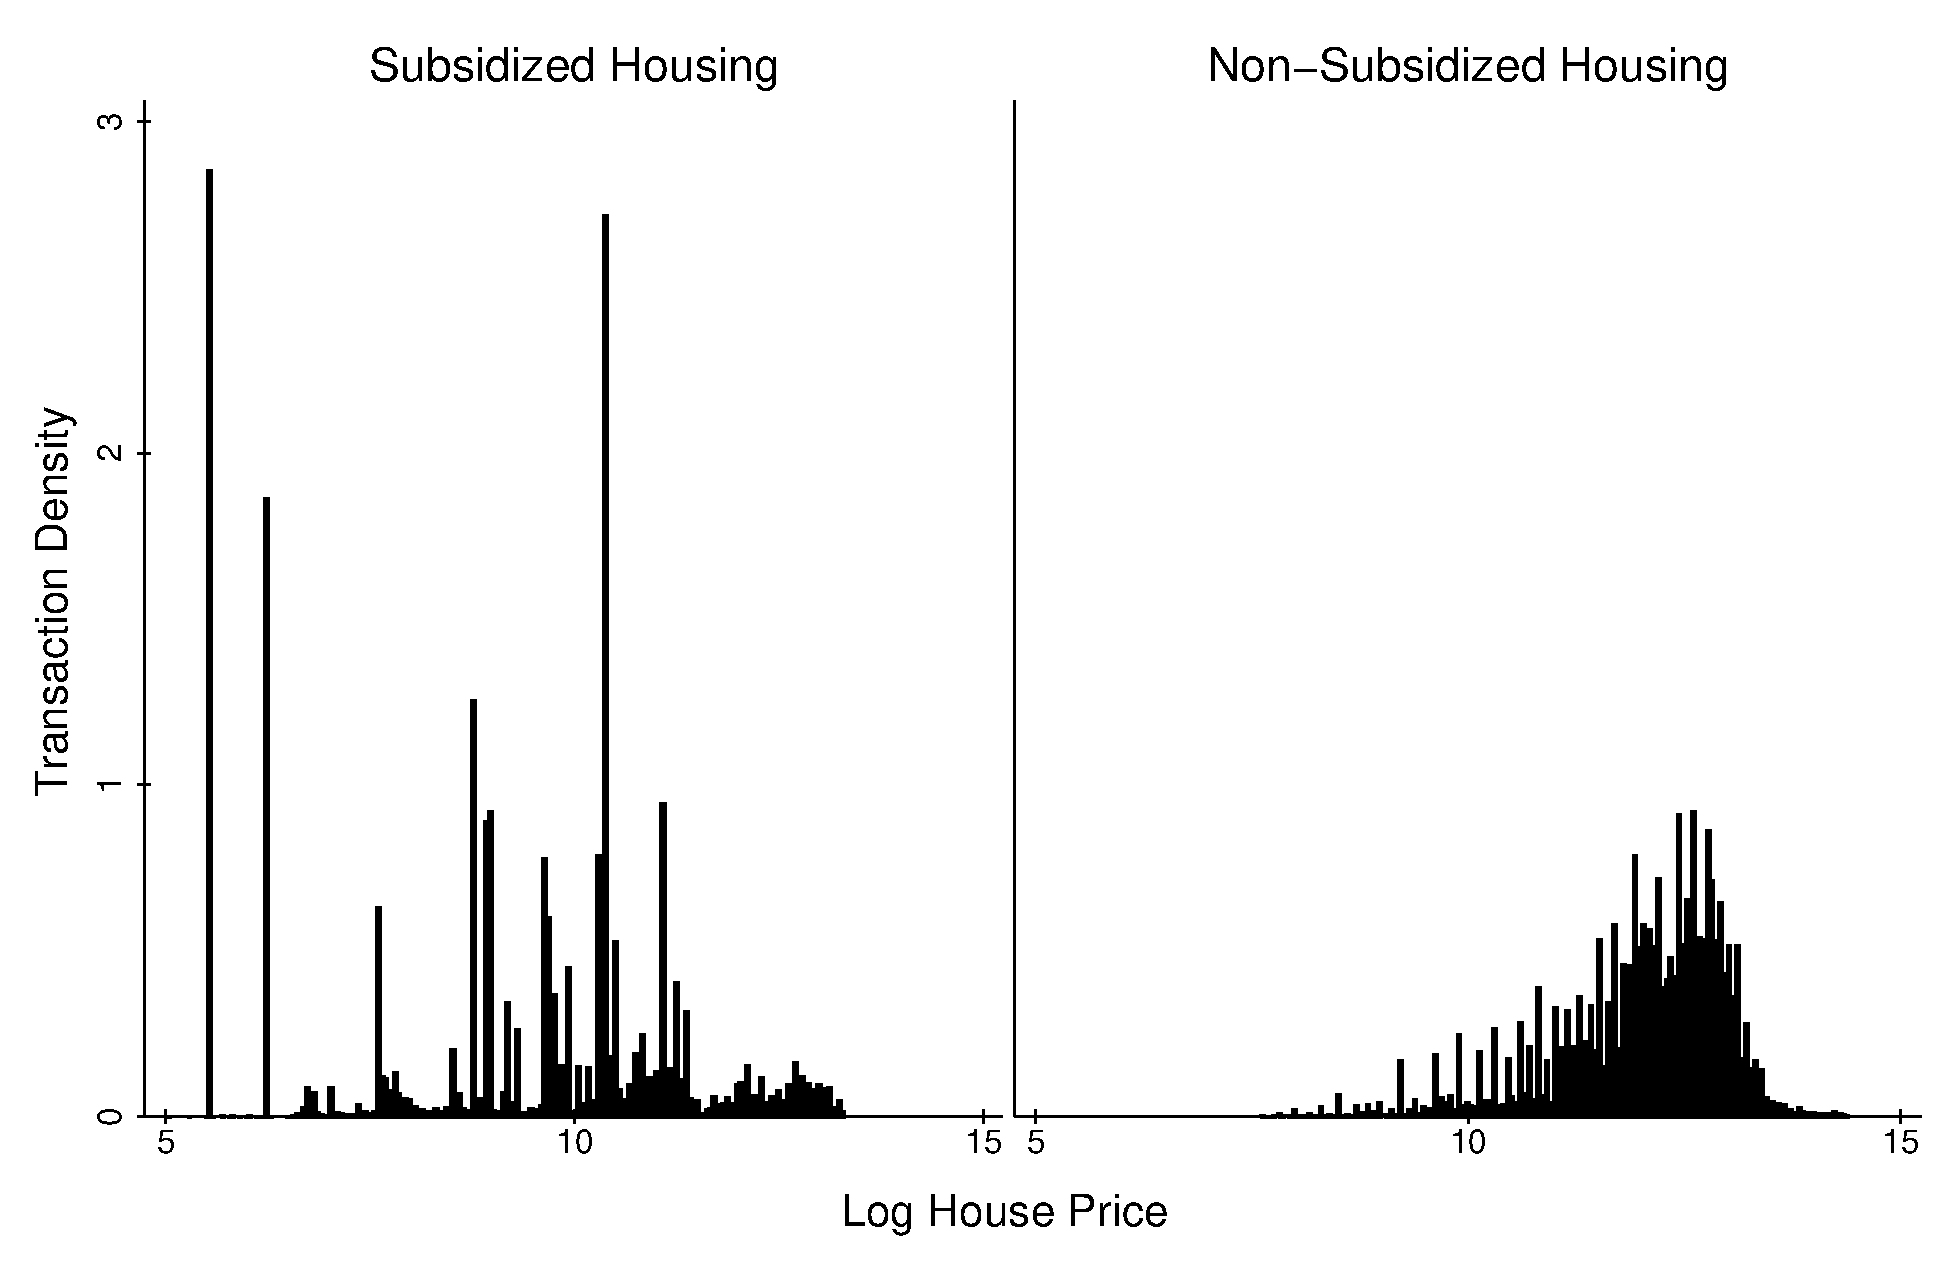
\includegraphics[scale=.4,trim={0cm 0cm -1cm 0cm}]{figures/summary_pricedist.pdf}}
% %\\
% %\footnotesize{Note: Transactions are censored at R100,000.}
% \end{figure}

\vspace{0mm}
\begin{table}[h!]
\centering
\caption{Housing Project Areas Description}\label{table:projectdescriptives}
\vspace{0mm}
\begin{tabular}{l*{1}{cccccc}}
\toprule
  & \multicolumn{2}{c}{\textbf{All}}& \multicolumn{2}{c}{\textbf{City}}  & \multicolumn{2}{c}{\textbf{Suburb}}   \\
  &Const. & Unconst. &Const. & Unconst.   & Const. & Unconst. \\
\midrule
 Number of Projects  & 72  & 90  & 36  & 43  & 36  & 47  \\ 
 Area (km2)  & 5.62  & 2.36  & 4.34  & 2.15  & 6.90  & 2.55  \\ 
 Median Construction Yr.  & 2005  & 2006  & 2006  & 2006  & 2005  & 2007  \\ 
 Delivered Houses  & 895  & 0  & 1,310  & 0  & 480  & 0  \\ 
 House Price in 1 km (R$^\dagger$)  & 201,927  & 225,735  & 233,553  & 243,722  & 172,058  & 209,278  \\ 
 Distance to CBD$^\ddagger$ (km)  & 31.9  & 33.1  & 22.8  & 23.0  & 41.0  & 42.4  \\ 

\bottomrule
\multicolumn{7}{l}{\scriptsize Const. refers to constructed projects and unconst. refers to unconstructed projects.}\\[-.5em]
\multicolumn{7}{l}{\scriptsize $^*$Calculated from {\it expected} completion dates using Gauteng National Treasury budget reports.}\\[-.5em]
\multicolumn{7}{l}{\scriptsize $^\dagger$ The USD averaged to about 7.70 Rands during the 2001-2011 period.}\\[-.5em]
\multicolumn{7}{l}{\scriptsize $^\ddagger$Measured as the average minimum distance with respect to Johannesburg and Pretoria CBDs. } \\[-.5em]
\multicolumn{7}{l}{\scriptsize City includes projects whose centroids are within 30.4 km of their nearest CBD.} \\[-.5em]
\multicolumn{7}{l}{\scriptsize Suburb includes projects whose centroids are further than 30.4 km from their nearest CBD.}
\end{tabular}
\end{table} 



\begin{table}[h!]
	\centering
	\caption{Dwelling Characteristics at Baseline from 2001 Census}\label{table:projectdescriptivescensus}
\vspace{-2mm}
\begin{tabular}{l*{1}{ccc}}
\toprule
& Constructed & Unconstructed & All Small Areas \\
\midrule
Flush Toilet&0.52&0.41&0.76 \\
Piped Water in Home&0.12&0.21&0.37 \\
Electricity for Cooking&0.32&0.38&0.67 \\
Electricity for Heating&0.29&0.37&0.65 \\
Electricity for Lighting&0.55&0.51&0.78 \\
Number of Rooms&2.88&2.59&3.51 \\
Household Size&3.53&3.22&3.53 \\
N&          1,303&            359&          7,350 \\
 
\bottomrule
\multicolumn{4}{l}{\scriptsize ``Constructed'' and ``Unconstructed'' include census small-areas with over 30\% } \\ [-.5em]
\multicolumn{4}{l}{\scriptsize  area overlap with constructed and unconstructed projects respectively. } \\ [-.5em]
\multicolumn{4}{l}{\scriptsize ``All''  includes all small areas.}
\end{tabular}
\end{table}



\begin{figure*}[h!]
        \centering
        \caption[ Pre-Period Housing Densities in Constructed and Unconstructed Projects Areas ]
        {\small Pre-Period Housing Densities in Constructed and Unconstructed projects } 
        %\vspace{2mm}
        \begin{subfigure}[b]{0.495\textwidth}
            \centering
            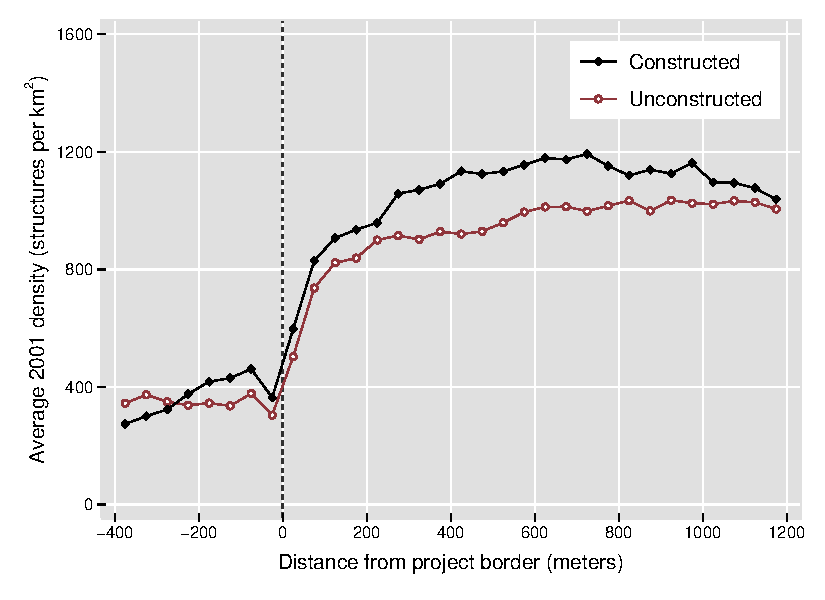
\includegraphics[width=\textwidth,trim={0.3cm .3cm 0.1cm 0cm}, clip=true]{figures/bblu_for_pre_means_2}
            \caption[Network2]%
            {{\small pre-period formal housing density}}    
            \label{fig:prefor}
        \end{subfigure}
        \hfill
        \begin{subfigure}[b]{0.495\textwidth}  
            \centering 
            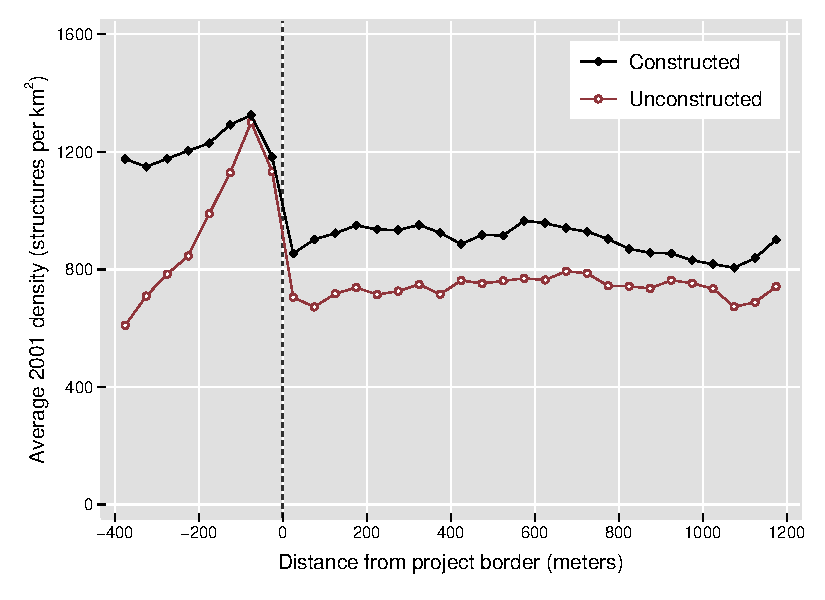
\includegraphics[width=\textwidth,trim={0.3cm .3cm 0.1cm 0cm}, clip=true]{figures/bblu_inf_pre_means_2}
            \caption[]%
            {{\small pre-period informal housing density}}    
            \label{fig:preinf}
        \end{subfigure}
        \label{fig:rawbblumeans}
        \vspace{-6mm}
    \end{figure*} 


\begin{figure*}[h!]
        \centering
        \caption[ Pre-Period Housing Densities in Constructed and Unconstructed Projects: City versus Suburb]
        {\small Pre-Period Housing Densities in Constructed and Unconstructed Projects: City versus Suburb} 
        %\vspace{2mm}
        \begin{subfigure}[b]{0.495\textwidth}
            \centering
            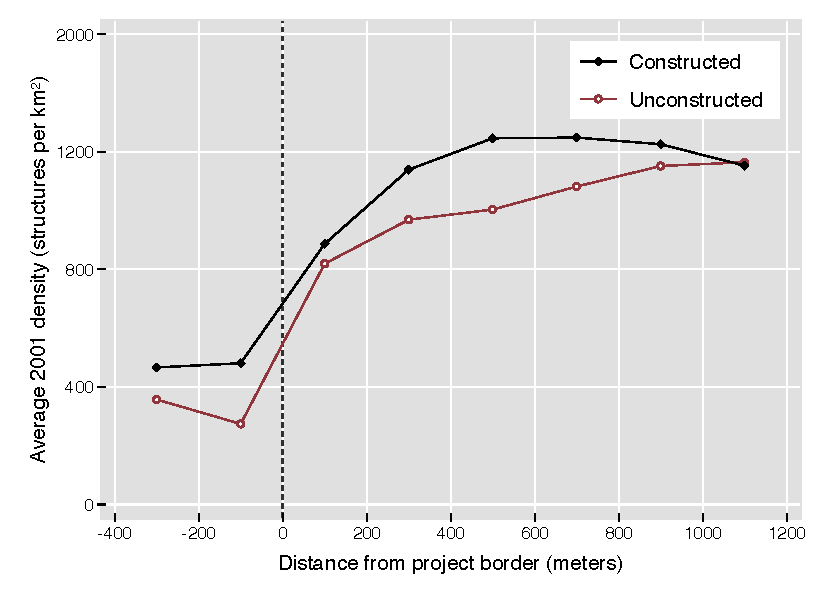
\includegraphics[width=\textwidth,trim={0.3cm .3cm 0.1cm 0cm}, clip=true]{figures/bblu_for_pre_means_het_near_2.pdf}
            \caption[Network2]%
            {{\small \textbf{City:} formal density}}    
            \label{fig:prefor_near_het}
        \end{subfigure}
        \hfill
        \begin{subfigure}[b]{0.495\textwidth}  
            \centering 
            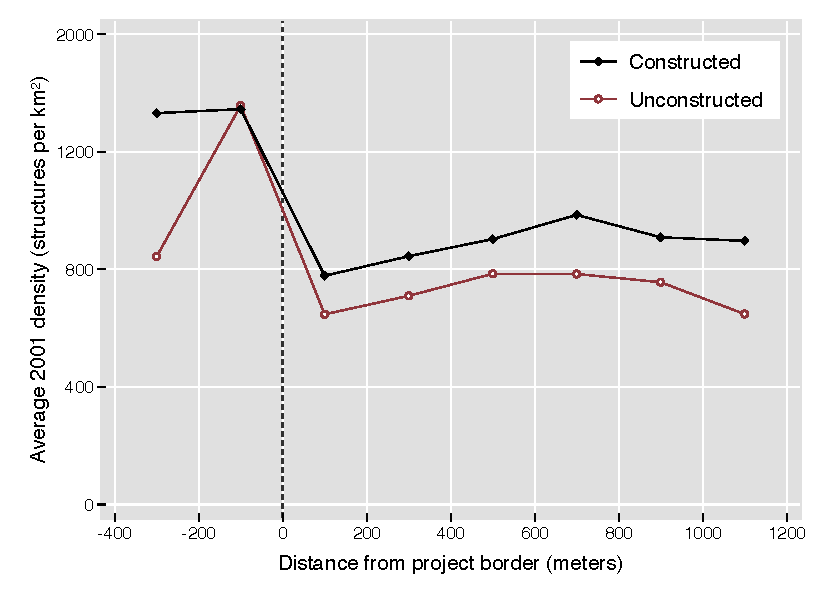
\includegraphics[width=\textwidth,trim={0.3cm .3cm 0.1cm 0cm}, clip=true]{figures/bblu_inf_pre_means_het_near_2.pdf}
            \caption[]%
            {{\small \textbf{City:} informal density}}    
            \label{fig:preinf_near_het}
        \end{subfigure}
        \begin{subfigure}[b]{0.495\textwidth}
            \centering
            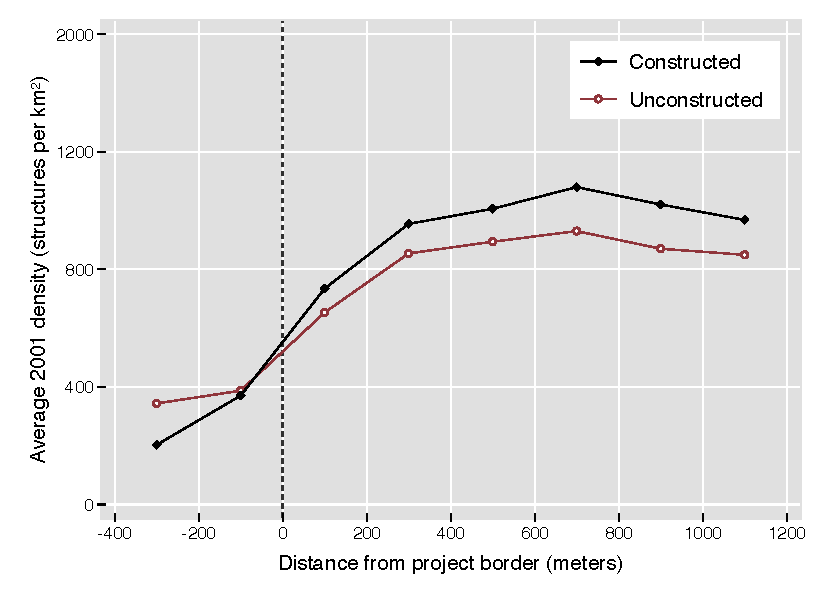
\includegraphics[width=\textwidth,trim={0.3cm .3cm 0.1cm 0cm}, clip=true]{figures/bblu_for_pre_means_het_far_2.pdf}
            \caption[Network2]%
            {{\small \textbf{Suburb:} formal density}}    
            \label{fig:prefor_far_het}
        \end{subfigure}
        \hfill
        \begin{subfigure}[b]{0.495\textwidth}  
            \centering 
            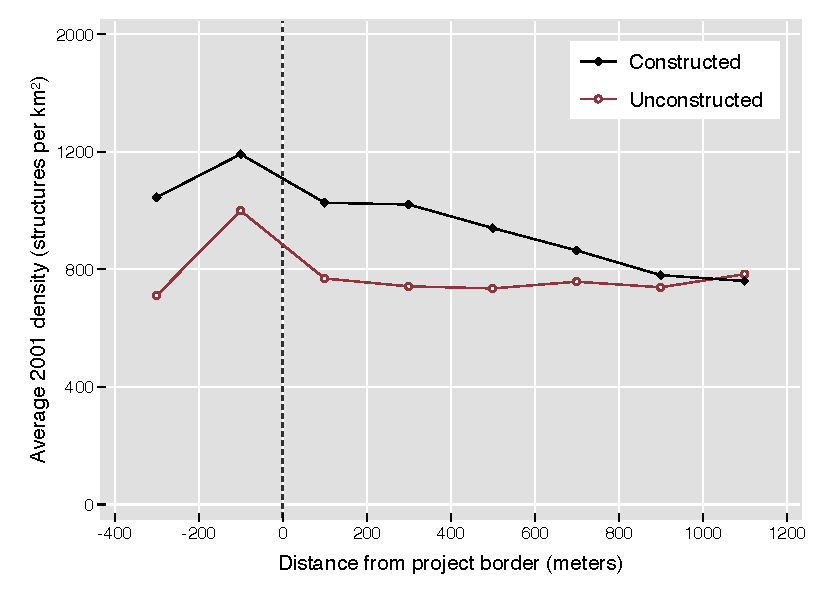
\includegraphics[width=\textwidth,trim={0.3cm .3cm 0.1cm 0cm}, clip=true]{figures/bblu_inf_pre_means_het_far_2.pdf}
            \caption[]%
            {{\small \textbf{Suburb:} informal density}}    
            \label{fig:preinf_far_het}
        \end{subfigure}
        \label{fig:rawbblumeans_het}
        \vspace{-6mm}
    {\scriptsize City includes areas within 30.4 km of a CBD and Suburb includes areas over 30.4 km away from a CBD.}
    \end{figure*} 



\begin{figure*}[t!]
        \centering
        \caption[ Changes in Housing Densities in Constructed and Unconstructed Projects Areas]
        {\small Housing Densities in Constructed and Unconstructed projects } 
        %\vspace{2mm}
        \begin{subfigure}[b]{0.495\textwidth}   
            \centering 
            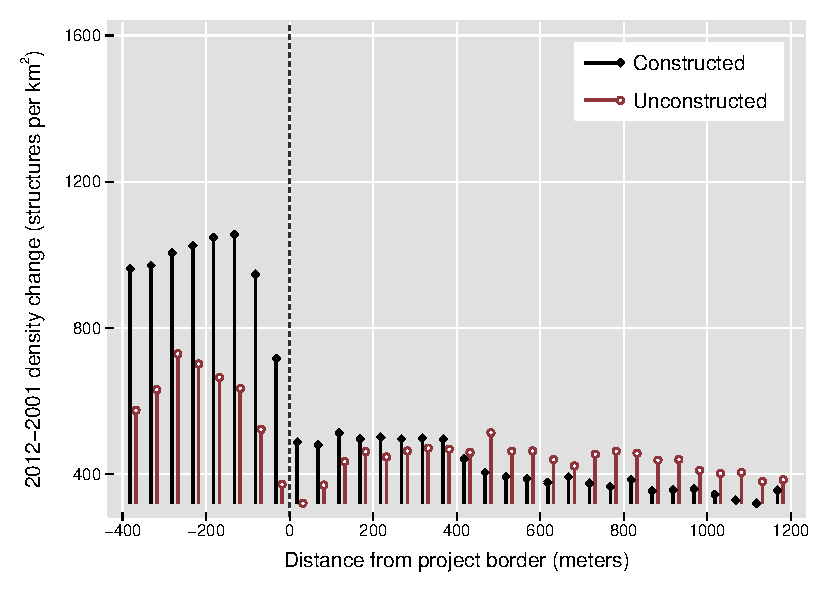
\includegraphics[width=\textwidth,trim={0.3cm .3cm 0.1cm 0cm}, clip=true]{figures/bblu_for_rawchanges_2}
            \caption[]%
            {{\small formal housing density change}}    
            \label{fig:forchange}
        \end{subfigure}
        \hfill
        \begin{subfigure}[b]{0.495\textwidth}   
            \centering 
            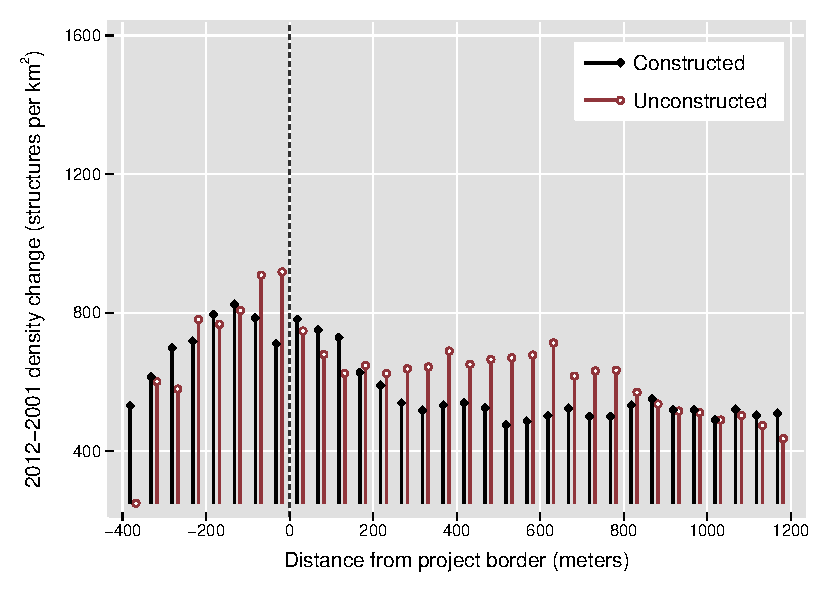
\includegraphics[width=\textwidth,trim={0.3cm .3cm 0.1cm 0cm}, clip=true]{figures/bblu_inf_rawchanges_2}
            \caption[]%
            {{\small informal housing density change}}    
            \label{fig:infchange}
        \end{subfigure}
        \label{fig:rawbblumeanschange}
        \vspace{-6mm}
    \end{figure*} 


% \begin{figure*}[t!]
%         \centering
%         \caption[ House Prices outside Constructed and Unconstructed Projects Areas ]
%         {\small House Prices outside Constructed and Unconstructed projects } 
%         %\vspace{2mm}
%         \begin{subfigure}[b]{0.495\textwidth}
%             \centering
%             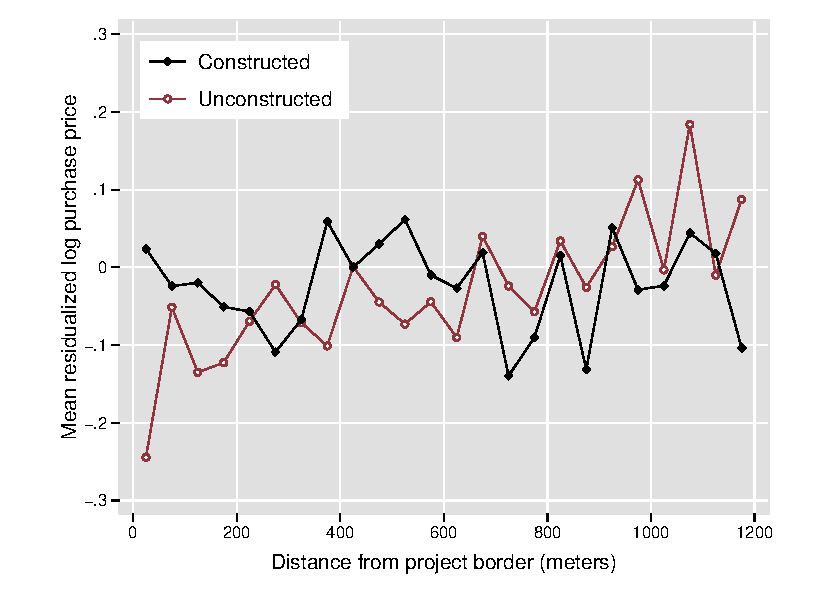
\includegraphics[width=\textwidth,trim={0.9cm .3cm 0.1cm 0cm}, clip=true]{figures/price_pre_means}
%             \caption[Network2]%
%             {{\small pre-period log-purchase prices }}    
%             \label{fig:preprice}
%         \end{subfigure}
%         \hfill
%         \begin{subfigure}[b]{0.495\textwidth}   
%             \centering 
%             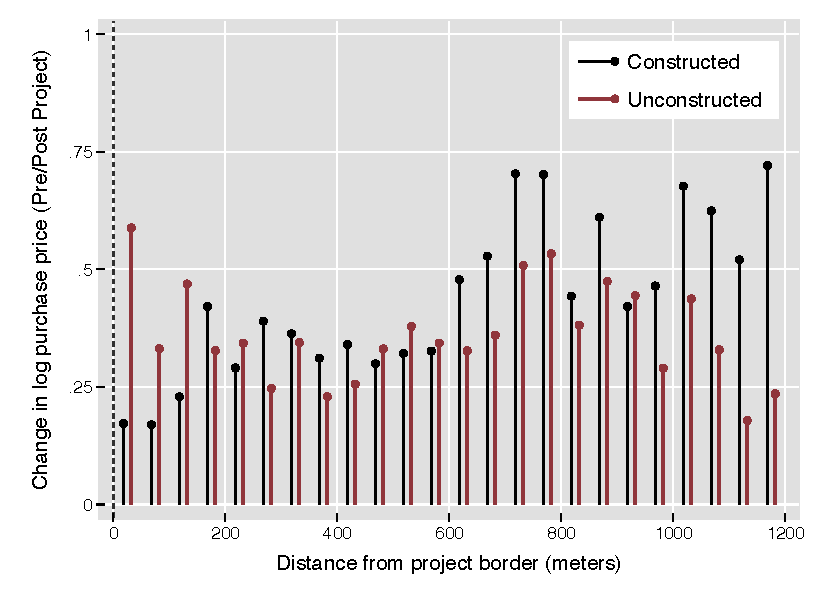
\includegraphics[width=\textwidth,trim={0.9cm .3cm 0.1cm 0cm}, clip=true]{figures/prices_rawchanges}
%             \caption[]%
%             {{\small change in log-purchase prices}}    
%             \label{fig:changeprice}
%         \end{subfigure}
%         \label{fig:rawpricemeans}
%         \vspace{-6mm}
% \end{figure*} 


\afterpage{%
  \clearpage% 
\begin{landscape}
{\footnotesize
\begin{table}[]
\small
\centering
\caption{Census Household-level Estimates}\label{table:censusestimates}
\vspace{-2mm}
\begin{tabular}{lDDDDDDDD}
\toprule
 & \small (1) & \small (2)  & \small (3) & \small (4) & \small (5)  & \small (6)  & \small (7) & (8)\\
 & \small Flush Toilet & \small Water Indoors  & \small Electricity Cooking & \small Electricity Heating & \small Electricity Lighting  & \small Number of Rooms  & \small Household Size & Population Density\\ \midrule 
project{\tim}post{\tim}constr&       0.094                   &       0.119\textsuperscript{a}&       0.215\textsuperscript{a}&       0.148\textsuperscript{b}&       0.087                   &      -0.211                   &      -0.305\textsuperscript{a}&     751.355                   \\
            &     (0.065)                   &     (0.042)                   &     (0.070)                   &     (0.060)                   &     (0.072)                   &     (0.136)                   &     (0.094)                   &   (902.093)                   \\[0.5em]
project{\tim}post&       0.086\textsuperscript{c}&       0.086\textsuperscript{b}&       0.197\textsuperscript{a}&       0.159\textsuperscript{a}&       0.125\textsuperscript{b}&       0.556\textsuperscript{a}&       0.043                   &    1642.578\textsuperscript{a}\\
            &     (0.045)                   &     (0.035)                   &     (0.057)                   &     (0.050)                   &     (0.059)                   &     (0.090)                   &     (0.050)                   &   (473.428)                   \\[0.5em]
project{\tim}constr&       0.074                   &      -0.087                   &      -0.030                   &      -0.009                   &       0.062                   &       0.302                   &       0.496\textsuperscript{a}&     165.664                   \\
            &     (0.088)                   &     (0.072)                   &     (0.071)                   &     (0.068)                   &     (0.086)                   &     (0.194)                   &     (0.113)                   &   (852.612)                   \\[0.5em]
project     &      -0.376\textsuperscript{a}&      -0.242\textsuperscript{a}&      -0.412\textsuperscript{a}&      -0.375\textsuperscript{a}&      -0.367\textsuperscript{a}&      -1.243\textsuperscript{a}&      -0.482\textsuperscript{a}&     126.982                   \\
            &     (0.067)                   &     (0.044)                   &     (0.052)                   &     (0.051)                   &     (0.066)                   &     (0.121)                   &     (0.078)                   &   (573.383)                   \\[0.5em]
spillover{\tim}post{\tim}constr&       0.037                   &       0.084\textsuperscript{a}&       0.070\textsuperscript{a}&       0.023                   &      -0.003                   &       0.082                   &      -0.172\textsuperscript{a}&     -45.080                   \\
            &     (0.027)                   &     (0.028)                   &     (0.027)                   &     (0.037)                   &     (0.023)                   &     (0.076)                   &     (0.045)                   &   (400.203)                   \\[0.5em]
spillover{\tim}post&       0.018                   &       0.111\textsuperscript{a}&       0.065\textsuperscript{a}&       0.040\textsuperscript{c}&       0.038\textsuperscript{c}&       0.201\textsuperscript{a}&      -0.134\textsuperscript{a}&     811.498\textsuperscript{b}\\
            &     (0.021)                   &     (0.021)                   &     (0.022)                   &     (0.022)                   &     (0.022)                   &     (0.055)                   &     (0.037)                   &   (365.348)                   \\[0.5em]
spillover{\tim}constr&      -0.063                   &      -0.104\textsuperscript{a}&      -0.074\textsuperscript{b}&      -0.039                   &      -0.020                   &      -0.274\textsuperscript{a}&       0.144\textsuperscript{b}&     577.695                   \\
            &     (0.042)                   &     (0.040)                   &     (0.035)                   &     (0.034)                   &     (0.036)                   &     (0.100)                   &     (0.057)                   &   (544.783)                   \\ \midrule
{\it p}-val, h\textsubscript{0}: project=spill. &       0.361                   &       0.416                   &       0.028                   &       0.041                   &       0.198                   &       0.017                   &       0.093                   &       0.301                   \\
Mean Outcome 2001&        0.71                   &        0.33                   &        0.61                   &        0.58                   &        0.75                   &        3.39                   &        3.60                   &    7,120.59                   \\
Mean Outcome 2011&        0.79                   &        0.52                   &        0.80                   &        0.70                   &        0.82                   &        3.65                   &        3.26                   &    8,743.91                   \\
R$^2$       &       0.388                   &       0.349                   &       0.398                   &       0.348                   &       0.332                   &       0.406                   &       0.444                   &       0.395                   \\
\# projects &         164                   &         164                   &         164                   &         164                   &         164                   &         164                   &         164                   &         164                   \\
N project areas&       4,901                   &       4,901                   &       4,901                   &       4,901                   &       4,901                   &       4,898                   &       4,902                   &       4,902                   \\
N spillover areas&       8,016                   &       8,016                   &       8,016                   &       8,016                   &       8,016                   &       8,002                   &       8,015                   &       8,018                   \\
N           &      12,917                   &      12,917                   &      12,917                   &      12,917                   &      12,917                   &      12,900                   &      12,917                   &      12,920                   \\

\bottomrule
\multicolumn{9}{l}{\footnotesize All regressions include project Fixed-Effects. Standard errors clustered at the project level in parenthesis. \textsuperscript{c} p$<$0.10,\textsuperscript{b} p$<$0.05,\textsuperscript{a} p$<$0.01 }
\end{tabular}
\end{table}
}
\end{landscape}
}


% \afterpage{%
%   \clearpage% 
% \begin{landscape}
% {\footnotesize
% \begin{table}[]
% \small
% \centering
% \caption{Census Household-level Post\tim\unskip Constructed Coefficients: City Versus Suburb}\label{table:censusestimateshet}
% \vspace{-2mm}
% \begin{tabular}{lDDDDDDDD}
% \toprule
%  & \small (1) & \small (2)  & \small (3) & \small (4) & \small (5)  & \small (6)  & \small (7) & (8)\\
%  & \small Flush Toilet & \small Water Indoors  & \small Electricity Cooking & \small Electricity Heating & \small Electricity Lighting  & \small Number of Rooms  & \small Household Size & Population Density\\ \midrule 
% near proj{\tim}post{\tim}constr&       0.118                   &       0.094                   &       0.215\textsuperscript{c}&       0.119                   &       0.029                   &      -0.198                   &      -0.374\textsuperscript{b}&     623.207                   \\
            &     (0.092)                   &     (0.081)                   &     (0.110)                   &     (0.098)                   &     (0.115)                   &     (0.264)                   &     (0.152)                   &  (2214.128)                   \\
near proj{\tim}post&       0.026                   &       0.138\textsuperscript{c}&       0.209\textsuperscript{b}&       0.203\textsuperscript{b}&       0.214\textsuperscript{c}&       0.543\textsuperscript{a}&      -0.023                   &    3453.190\textsuperscript{c}\\
            &     (0.072)                   &     (0.070)                   &     (0.104)                   &     (0.092)                   &     (0.109)                   &     (0.171)                   &     (0.089)                   &  (1994.725)                   \\
near proj{\tim}constr&       0.225                   &       0.136                   &       0.072                   &       0.093                   &       0.260                   &       0.329                   &       0.537\textsuperscript{a}&   -1882.714                   \\
            &     (0.144)                   &     (0.121)                   &     (0.158)                   &     (0.133)                   &     (0.161)                   &     (0.353)                   &     (0.176)                   &  (2637.951)                   \\
near proj   &      -0.374\textsuperscript{a}&      -0.305\textsuperscript{a}&      -0.454\textsuperscript{a}&      -0.428\textsuperscript{a}&      -0.469\textsuperscript{a}&      -1.309\textsuperscript{a}&      -0.460\textsuperscript{a}&     727.416                   \\
            &     (0.109)                   &     (0.057)                   &     (0.097)                   &     (0.088)                   &     (0.105)                   &     (0.209)                   &     (0.129)                   &  (1224.633)                   \\
near spill{\tim}post{\tim}constr&       0.021                   &      -0.006                   &      -0.046                   &      -0.124\textsuperscript{b}&      -0.090\textsuperscript{b}&       0.018                   &      -0.177\textsuperscript{a}&     873.022                   \\
            &     (0.043)                   &     (0.042)                   &     (0.038)                   &     (0.050)                   &     (0.036)                   &     (0.115)                   &     (0.060)                   &   (654.256)                   \\
near spill{\tim}post&       0.006                   &       0.150\textsuperscript{a}&       0.091\textsuperscript{a}&       0.069\textsuperscript{b}&       0.083\textsuperscript{b}&       0.240\textsuperscript{a}&      -0.159\textsuperscript{a}&     748.687                   \\
            &     (0.031)                   &     (0.036)                   &     (0.034)                   &     (0.029)                   &     (0.032)                   &     (0.082)                   &     (0.043)                   &   (499.875)                   \\
near spill{\tim}constr&      -0.001                   &      -0.015                   &       0.005                   &       0.034                   &       0.059                   &      -0.291\textsuperscript{c}&       0.150\textsuperscript{b}&    -921.948                   \\
            &     (0.070)                   &     (0.071)                   &     (0.059)                   &     (0.056)                   &     (0.067)                   &     (0.157)                   &     (0.071)                   &  (1912.722)                   \\
far proj{\tim}post{\tim}constr&       0.088                   &       0.220\textsuperscript{a}&       0.280\textsuperscript{a}&       0.218\textsuperscript{a}&       0.084                   &      -0.002                   &      -0.171\textsuperscript{c}&    -275.692                   \\
            &     (0.081)                   &     (0.044)                   &     (0.082)                   &     (0.079)                   &     (0.114)                   &     (0.222)                   &     (0.102)                   &   (295.380)                   \\
far proj{\tim}post&       0.115\textsuperscript{b}&       0.051                   &       0.163\textsuperscript{a}&       0.119\textsuperscript{b}&       0.092                   &       0.326\textsuperscript{c}&      -0.040                   &     956.996\textsuperscript{a}\\
            &     (0.046)                   &     (0.034)                   &     (0.048)                   &     (0.053)                   &     (0.061)                   &     (0.193)                   &     (0.072)                   &   (221.740)                   \\
far proj{\tim}constr&      -0.080                   &      -0.172\textsuperscript{b}&      -0.166                   &      -0.171\textsuperscript{c}&       0.026                   &       0.347                   &       0.457\textsuperscript{a}&     750.473                   \\
            &     (0.150)                   &     (0.085)                   &     (0.108)                   &     (0.099)                   &     (0.148)                   &     (0.383)                   &     (0.168)                   &   (810.360)                   \\
far proj    &      -0.256\textsuperscript{a}&      -0.180\textsuperscript{b}&      -0.253\textsuperscript{a}&      -0.214\textsuperscript{a}&      -0.260\textsuperscript{a}&      -0.807\textsuperscript{a}&      -0.344\textsuperscript{a}&      20.551                   \\
            &     (0.093)                   &     (0.072)                   &     (0.077)                   &     (0.069)                   &     (0.097)                   &     (0.257)                   &     (0.087)                   &   (486.387)                   \\
far spill{\tim}post{\tim}constr&       0.016                   &       0.122\textsuperscript{b}&       0.141\textsuperscript{a}&       0.098\textsuperscript{b}&       0.033                   &       0.097                   &      -0.118\textsuperscript{c}&    -221.692                   \\
            &     (0.057)                   &     (0.054)                   &     (0.037)                   &     (0.045)                   &     (0.036)                   &     (0.092)                   &     (0.070)                   &   (390.402)                   \\
far spill{\tim}post&       0.079\textsuperscript{b}&       0.108\textsuperscript{b}&       0.114\textsuperscript{a}&       0.099\textsuperscript{a}&       0.028                   &       0.262\textsuperscript{a}&      -0.156\textsuperscript{a}&     605.784\textsuperscript{c}\\
            &     (0.036)                   &     (0.048)                   &     (0.030)                   &     (0.034)                   &     (0.029)                   &     (0.068)                   &     (0.056)                   &   (349.145)                   \\
far spill{\tim}constr&      -0.047                   &      -0.097\textsuperscript{b}&      -0.118\textsuperscript{a}&      -0.097\textsuperscript{b}&      -0.006                   &       0.080                   &       0.202\textsuperscript{b}&    1122.421\textsuperscript{b}\\
            &     (0.051)                   &     (0.038)                   &     (0.034)                   &     (0.049)                   &     (0.031)                   &     (0.146)                   &     (0.082)                   &   (530.285)                   \\
{\it p}-val, h\textsubscript{0}: project=spill. &       0.354                   &       0.126                   &       0.088                   &       0.137                   &       0.640                   &       0.641                   &       0.637                   &       0.909                   \\
Mean Outcome 2001&        0.72                   &        0.31                   &        0.60                   &        0.57                   &        0.75                   &        3.31                   &        3.59                   &    7,313.26                   \\
Mean Outcome 2011&        0.79                   &        0.51                   &        0.80                   &        0.69                   &        0.82                   &        3.57                   &        3.22                   &    9,118.36                   \\
R$^2$       &       0.344                   &       0.324                   &       0.374                   &       0.329                   &       0.300                   &       0.370                   &       0.445                   &       0.407                   \\
\# projects &         117                   &         117                   &         117                   &         117                   &         117                   &         117                   &         117                   &         117                   \\
N project areas&       1,722                   &       1,722                   &       1,722                   &       1,722                   &       1,722                   &       1,722                   &       1,722                   &       1,722                   \\
N spillover areas&       2,306                   &       2,306                   &       2,306                   &       2,306                   &       2,306                   &       2,305                   &       2,307                   &       2,307                   \\
N           &       9,609                   &       9,609                   &       9,609                   &       9,609                   &       9,609                   &       9,594                   &       9,609                   &       9,612                   \\

% \bottomrule
% \multicolumn{9}{l}{\footnotesize All difference-in-differences controls are included in the specification while only the interaction terms for Post\tim Constructed are shown.} \\
% \multicolumn{9}{l}{\footnotesize All regressions include project Fixed-Effects. Standard errors clustered at the project level in parenthesis. \textsuperscript{c} p$<$0.10,\textsuperscript{b} p$<$0.05,\textsuperscript{a} p$<$0.01 }
% \end{tabular}
% \end{table}
% }
% \end{landscape}
% }




\afterpage{%
  \clearpage% 
\begin{landscape}
{\footnotesize
\begin{table}[]
\small
\centering
\caption{Census Household-level Post\tim\unskip Constructed Coefficients: City Versus Suburb and Informal Versus Formal Housing}\label{table:censusestimates_dwellhet}
\vspace{-2mm}
\begin{tabular}{lDDDDDDDD}
\toprule
% & \small (1) & \small (2)  & \small (3) & \small (4) & \small (5)  & \small (6)  & \small (7) & (8)\\

 & \small Flush Toilet & \small Water Indoors  & \small Electricity Cooking & \small Electricity Heating & \small Electricity Lighting  & \small Number of Rooms  & \small Household Size & Population Density\\
  & \multicolumn{8}{c}{ } \\
 & \multicolumn{8}{c}{Formal Houses} \\ \midrule 
City{\tim}proj&       0.050                   &       0.119                   &       0.240\textsuperscript{a}&       0.150\textsuperscript{c}&       0.139                   &      -0.173                   &      -0.226                   &    1741.403                   \\
            &     (0.108)                   &     (0.081)                   &     (0.089)                   &     (0.083)                   &     (0.089)                   &     (0.231)                   &     (0.189)                   &  (1201.688)                   \\[0.5em]
City{\tim}spill&      -0.009                   &       0.055                   &       0.004                   &      -0.063                   &      -0.025                   &       0.039                   &      -0.143\textsuperscript{b}&    -196.705                   \\
            &     (0.028)                   &     (0.037)                   &     (0.027)                   &     (0.041)                   &     (0.027)                   &     (0.079)                   &     (0.068)                   &   (610.402)                   \\[0.5em]
Suburb{\tim}proj&       0.127\textsuperscript{c}&       0.162\textsuperscript{a}&       0.175\textsuperscript{c}&       0.142\textsuperscript{c}&       0.033                   &      -0.264                   &      -0.288\textsuperscript{b}&    -336.118                   \\
            &     (0.072)                   &     (0.059)                   &     (0.095)                   &     (0.080)                   &     (0.108)                   &     (0.198)                   &     (0.111)                   &   (459.638)                   \\[0.5em]
Suburb{\tim}spill&       0.080                   &       0.142\textsuperscript{a}&       0.135\textsuperscript{a}&       0.120\textsuperscript{a}&       0.007                   &       0.125                   &      -0.208\textsuperscript{a}&     -31.393                   \\
            &     (0.049)                   &     (0.041)                   &     (0.034)                   &     (0.034)                   &     (0.031)                   &     (0.106)                   &     (0.069)                   &   (271.422)                   \\[0.5em]

  & \multicolumn{8}{c}{ } \\
 & \multicolumn{8}{c}{Informal Houses} \\ \midrule 
% & \small (1) & \small (2)  & \small (3) & \small (4) & \small (5)  & \small (6)  & \small (7) & (8)\\
% & \small Flush Toilet & \small Water Indoors  & \small Electricity Cooking & \small Electricity Heating & \small Electricity Lighting  & \small Number of Rooms  & \small Household Size & Population Density\\ \midrule 
City{\tim}proj&       0.086                   &       0.092\textsuperscript{c}&       0.281\textsuperscript{a}&       0.174\textsuperscript{b}&       0.171\textsuperscript{b}&      -0.519\textsuperscript{a}&      -0.507\textsuperscript{a}&    1531.549                   \\
            &     (0.099)                   &     (0.050)                   &     (0.092)                   &     (0.078)                   &     (0.085)                   &     (0.138)                   &     (0.115)                   &  (1241.915)                   \\[0.5em]
City{\tim}spill&      -0.002                   &       0.044\textsuperscript{c}&       0.036                   &      -0.041                   &      -0.003                   &      -0.131                   &      -0.188\textsuperscript{a}&     -70.920                   \\
            &     (0.034)                   &     (0.024)                   &     (0.033)                   &     (0.046)                   &     (0.033)                   &     (0.102)                   &     (0.060)                   &   (657.012)                   \\[0.5em]
Suburb{\tim}proj&       0.045                   &       0.088\textsuperscript{c}&       0.109                   &       0.080                   &      -0.024                   &      -0.389\textsuperscript{a}&      -0.295\textsuperscript{a}&    -200.174                   \\
            &     (0.071)                   &     (0.047)                   &     (0.088)                   &     (0.077)                   &     (0.107)                   &     (0.113)                   &     (0.100)                   &   (483.756)                   \\[0.5em]
Suburb{\tim}spill&       0.084\textsuperscript{b}&       0.089\textsuperscript{a}&       0.176\textsuperscript{a}&       0.166\textsuperscript{a}&       0.057\textsuperscript{c}&      -0.014                   &      -0.205\textsuperscript{a}&      63.607                   \\
            &     (0.040)                   &     (0.033)                   &     (0.036)                   &     (0.041)                   &     (0.031)                   &     (0.076)                   &     (0.067)                   &   (273.235)                   \\[0.5em]


\bottomrule
\multicolumn{9}{l}{\footnotesize All difference-in-differences controls are included in the specification while only the interaction terms for Post\tim Constructed are shown.} \\
\multicolumn{9}{l}{\footnotesize All regressions include project Fixed-Effects. Standard errors clustered at the project level in parenthesis. \textsuperscript{c} p$<$0.10,\textsuperscript{b} p$<$0.05,\textsuperscript{a} p$<$0.01 }
\end{tabular}
\end{table}
}
\end{landscape}
}


\begin{table}[h!] 
\caption{Effect of Housing Projects on Socio-demographics}
\label{table:sorting}
\small
\centering
%\caption{Census Composition Estimates }
\vspace{-2mm}
\begin{tabular}{lDDDDD}
\toprule
& \small (1) & \small (2) & \small (3) & \small (4)& \small (5)\\
& \small Age & \small P.O.B. not Gauteng & \small Unemployed & \small Years of Education & \small Monthly Income \\ \midrule 
project{\tim}post{\tim}constr&       0.078                   &      -0.002                   &      -0.020                   &       0.446\textsuperscript{a}&      12.817                   \\
            &     (0.258)                   &     (0.061)                   &     (0.020)                   &     (0.154)                   &   (379.729)                   \\[0.5em]
project{\tim}post&       0.740\textsuperscript{a}&      -0.059\textsuperscript{c}&      -0.111\textsuperscript{a}&       1.072\textsuperscript{a}&     231.513                   \\
            &     (0.228)                   &     (0.033)                   &     (0.015)                   &     (0.117)                   &   (288.752)                   \\[0.5em]
project{\tim}constr&      -0.804\textsuperscript{b}&      -0.034                   &      -0.000                   &      -0.442\textsuperscript{b}&    -120.973                   \\
            &     (0.378)                   &     (0.041)                   &     (0.021)                   &     (0.177)                   &   (505.906)                   \\[0.5em]
project     &      -1.670\textsuperscript{a}&       0.193\textsuperscript{a}&       0.109\textsuperscript{a}&      -1.076\textsuperscript{a}&   -1312.384\textsuperscript{a}\\
            &     (0.225)                   &     (0.030)                   &     (0.014)                   &     (0.119)                   &   (288.124)                   \\[0.5em]
spillover{\tim}post{\tim}constr&       0.589\textsuperscript{a}&      -0.007                   &      -0.069\textsuperscript{a}&       0.450\textsuperscript{a}&     237.912                   \\
            &     (0.204)                   &     (0.023)                   &     (0.014)                   &     (0.096)                   &   (359.015)                   \\[0.5em]
spillover{\tim}post&       1.001\textsuperscript{a}&       0.017                   &      -0.065\textsuperscript{a}&       0.847\textsuperscript{a}&    1818.611\textsuperscript{a}\\
            &     (0.155)                   &     (0.012)                   &     (0.010)                   &     (0.078)                   &   (293.202)                   \\[0.5em]
spillover{\tim}constr&      -1.239\textsuperscript{a}&       0.016                   &       0.060\textsuperscript{a}&      -0.567\textsuperscript{a}&    -923.554\textsuperscript{a}\\
            &     (0.247)                   &     (0.021)                   &     (0.016)                   &     (0.087)                   &   (331.983)                   \\ \midrule
{\it p}-val, h\textsubscript{0}: project=spill. &       0.101                   &       0.913                   &       0.006                   &       0.984                   &       0.591                   \\
Mean Outcome 2001&       26.72                   &        0.41                   &        0.47                   &        8.12                   &    2,378.40                   \\
Mean Outcome 2011&       27.92                   &        0.43                   &        0.33                   &        9.57                   &    4,211.81                   \\
R$^2$       &       0.406                   &       0.521                   &       0.300                   &       0.525                   &       0.351                   \\
\# projects &         164                   &         164                   &         164                   &         164                   &         164                   \\
N project areas&       4,902                   &       4,901                   &       4,900                   &       4,900                   &       4,900                   \\
N spillover areas&       8,013                   &       8,009                   &       8,005                   &       8,009                   &       8,007                   \\
N           &      12,915                   &      12,910                   &      12,905                   &      12,909                   &      12,907                   \\

\bottomrule
\multicolumn{6}{l}{\footnotesize Standard errors clustered at the project level in parenthesis. \textsuperscript{c} p$<$0.10, \textsuperscript{b} p$<$0.05, \textsuperscript{a} p$<$0.01  }\\
\multicolumn{6}{l}{\footnotesize P.O.B. means ``place of birth.''  Monthly income is in Rands.}
\end{tabular}
\end{table}


\begin{table}[h!] 
\caption{Census Household-level Post\tim\unskip Constructed Coefficients: City Versus Suburb}
\label{table:sorting_het}
\small
\centering
%\caption{Census Composition Estimates }
\vspace{-2mm}
\begin{tabular}{lDDDDD}
\toprule
& \small (1) & \small (2) & \small (3) & \small (4)& \small (5)\\
& \small Age & \small P.O.B. not Gauteng & \small Unemployed & \small Years of Education & \small Monthly Income \\ \midrule 
City{\tim}proj&       0.091                   &       0.050                   &      -0.051                   &       0.674\textsuperscript{a}&     849.026                   \\
            &     (0.299)                   &     (0.035)                   &     (0.033)                   &     (0.213)                   &   (706.540)                   \\[0.5em]
City{\tim}spill&       0.482\textsuperscript{c}&       0.014                   &      -0.060\textsuperscript{a}&       0.466\textsuperscript{a}&     312.213                   \\
            &     (0.263)                   &     (0.021)                   &     (0.020)                   &     (0.130)                   &   (526.047)                   \\[0.5em]
Suburb{\tim}proj&       0.067                   &      -0.060                   &       0.005                   &       0.230                   &    -578.037\textsuperscript{b}\\
            &     (0.405)                   &     (0.101)                   &     (0.021)                   &     (0.184)                   &   (222.902)                   \\[0.5em]
Suburb{\tim}spill&       0.764\textsuperscript{b}&      -0.040                   &      -0.083\textsuperscript{a}&       0.429\textsuperscript{a}&     111.417                   \\
            &     (0.311)                   &     (0.038)                   &     (0.017)                   &     (0.121)                   &   (354.339)                   \\[1em]
{\it p}-val, h\textsubscript{0} City:  proj = spill &       0.315                   &       0.226                   &       0.708                   &       0.343                   &       0.465                   \\
{\it p}-val, h\textsubscript{0} Suburb: proj = spill &       0.118                   &       0.794                   &       0.000                   &       0.318                   &       0.039                   \\
R$^2$       &       0.408                   &       0.531                   &       0.300                   &       0.526                   &       0.356                   \\
N City proj areas&       2,546                   &       2,545                   &       2,544                   &       2,544                   &       2,544                   \\
N City spill areas&       4,739                   &       4,735                   &       4,734                   &       4,736                   &       4,735                   \\
N Suburb proj areas&       2,356                   &       2,356                   &       2,356                   &       2,356                   &       2,356                   \\
N Suburb spill areas&       3,274                   &       3,274                   &       3,271                   &       3,273                   &       3,272                   \\

\bottomrule
\multicolumn{6}{l}{\footnotesize All difference-in-differences controls are included in the specification while only the interaction terms} \\
\multicolumn{6}{l}{\footnotesize  for Post\tim Constructed are shown. Standard errors clustered at the project level in parenthesis.  }\\
\multicolumn{6}{l}{\footnotesize \textsuperscript{c} p$<$0.10, \textsuperscript{b} p$<$0.05, \textsuperscript{a} p$<$0.01. P.O.B. means ``place of birth.''  Monthly income is in Rands.}
\end{tabular}
\end{table}



%(2) differential shocks to local housing markets for constructed versus unconstructed projects are uncorrelated with distance within this radius, and (3) recipient households are not drawn from households living at 1,200 meters from the project area.

\begin{figure*}[t!]
    \centering
    \vspace{2mm}
    \begin{subfigure}[b]{0.49\textwidth}
        \centering
        \caption[]{\small Total Houses}  
        \vspace{-1mm}
        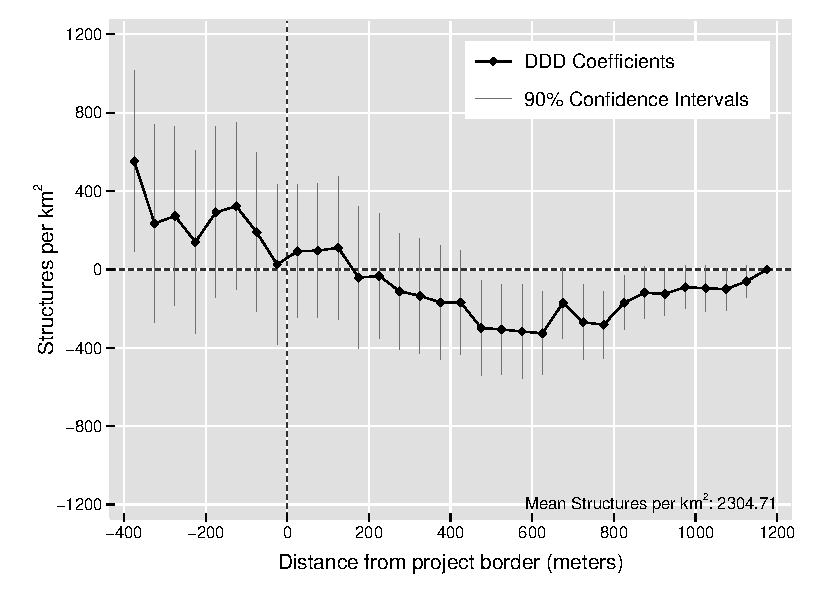
\includegraphics[width=\textwidth,trim={.5cm .3cm .3cm 0cm}, clip=true]{figures/distplotDDD_bblu_total_buildings_admin_2}
        \label{fig:DDDtotal}
    \end{subfigure}
    \hfill
    \begin{subfigure}[b]{0.49\textwidth}  
        \centering 
        \caption[]{\small Formal Houses}
        \vspace{-1mm}
        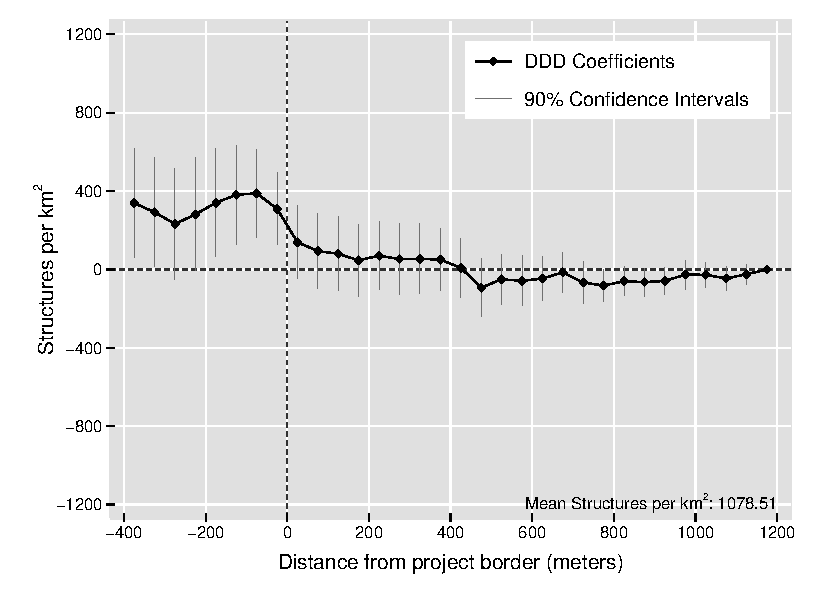
\includegraphics[width=\textwidth,trim={.5cm .3cm .3cm 0cm}, clip=true]{figures/distplotDDD_bblu_for_admin_2}     
        \label{fig:DDDformal}
    \end{subfigure}
    \vskip 1mm \vskip 0pt
    \begin{subfigure}[b]{0.49\textwidth}
        \centering
        \caption[]{\small Informal Houses}
        \vspace{-1mm}
        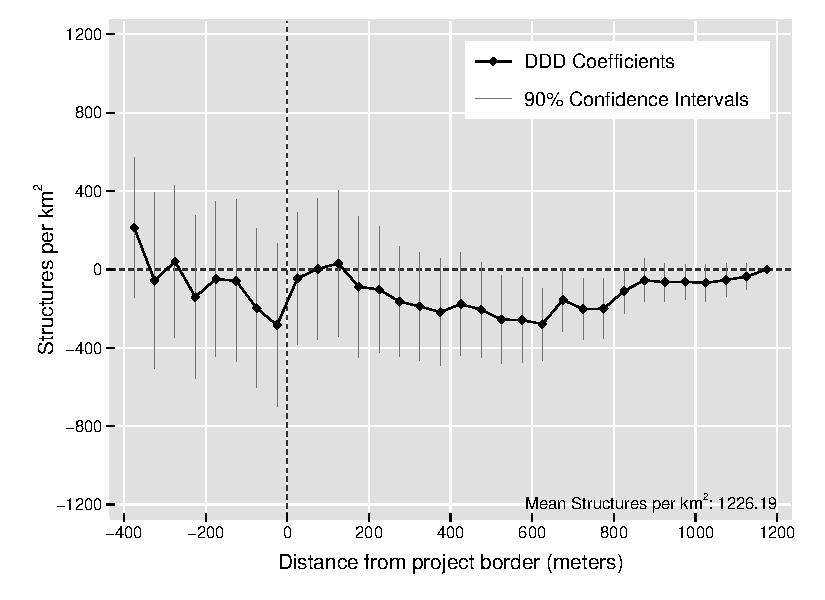
\includegraphics[width=\textwidth,trim={.5cm .3cm .3cm 0cm}, clip=true]{figures/distplotDDD_bblu_inf_admin_2.pdf}
        \label{fig:DDDinformal}
    \end{subfigure}
    \hfill
    \begin{subfigure}[b]{0.49\textwidth}  
        \centering
        \caption[]{\small Backyard Informal Houses}  
        \vspace{-1mm}
        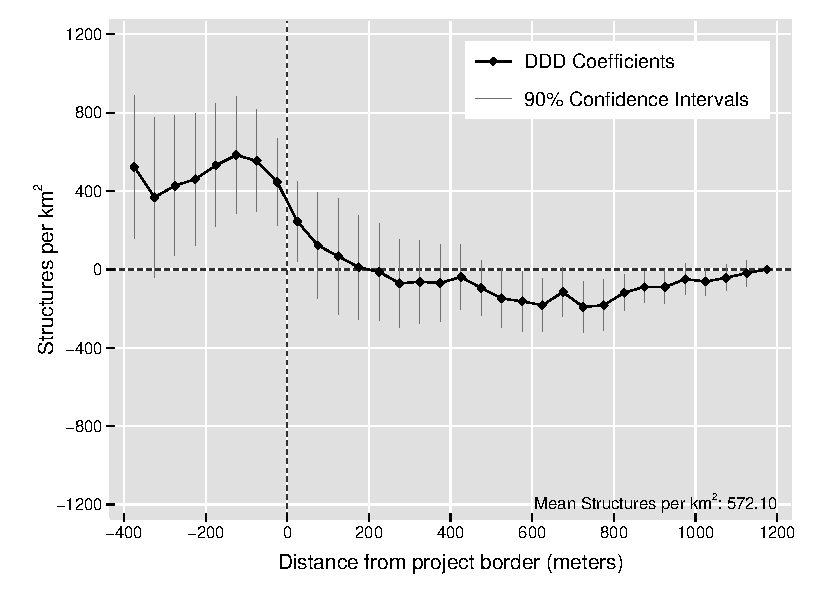
\includegraphics[width=\textwidth,trim={.5cm .3cm .3cm 0cm}, clip=true]{figures/distplotDDD_bblu_inf_backyard_admin_2}
        \label{fig:DDDbackyard}
    \end{subfigure}
    \vskip 1mm \vskip 0pt
    \begin{subfigure}[b]{.49\textwidth}  
        \centering
        \caption[]{\small Non-Backyard Informal Houses} 
        \vspace{-1mm}
        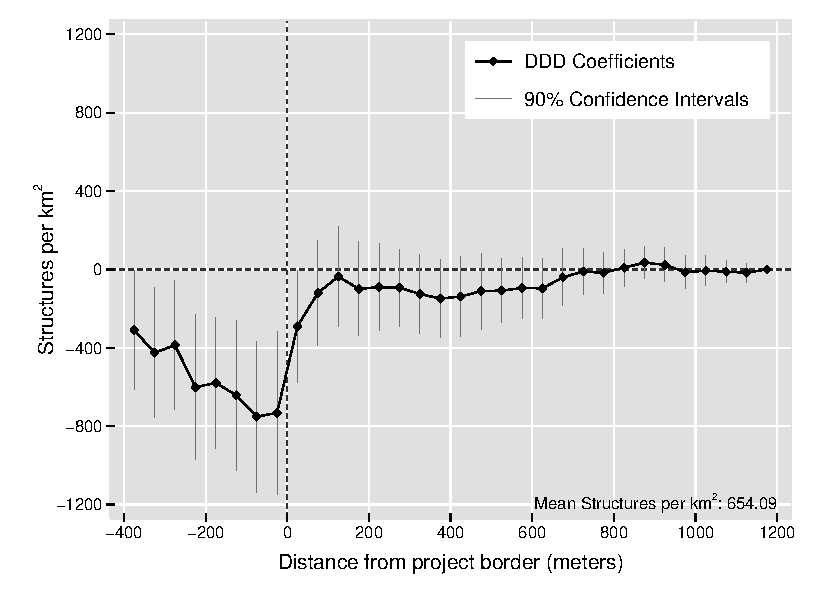
\includegraphics[width=\textwidth,trim={.5cm .3cm .3cm 0cm}, clip=true]{figures/distplotDDD_bblu_inf_non_backyard_admin_2}    
        \label{fig:DDDnonbackyard}
    \end{subfigure}
    \hfill \hspace{.02\textwidth}
    \begin{minipage}{0.47\textwidth}   
    \vspace{-6cm}
    \caption[]
    {\small DDD coefficients (equation \ref{eq:bblu}) for fives types of housing densities.} \label{fig:DDDbblu}
	\end{minipage}
\end{figure*} 




\begin{figure*}[t!]
    \centering
    \vspace{2mm}
    \begin{subfigure}[b]{0.49\textwidth}
        \centering
        \caption[]{\small Total Houses}  
        \vspace{-1mm}
        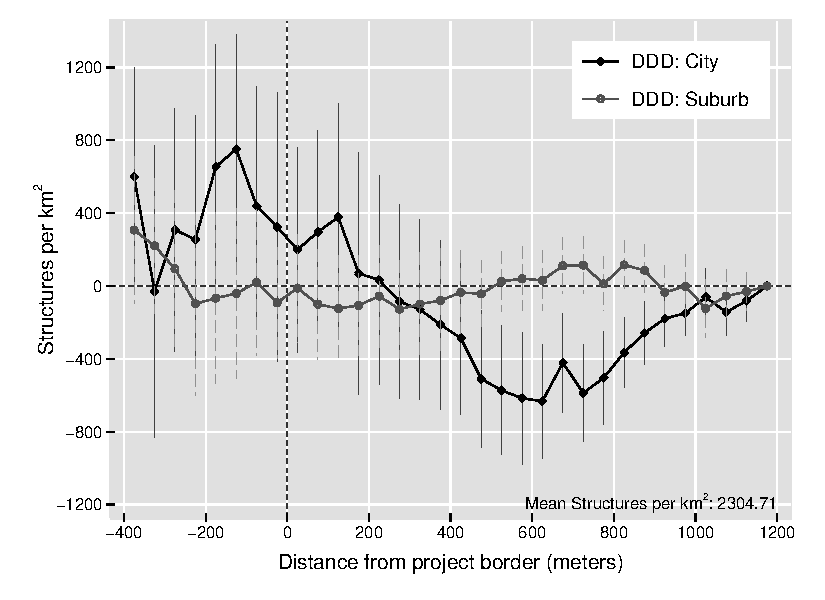
\includegraphics[width=\textwidth,trim={.5cm .3cm .3cm 0cm}, clip=true]{figures/distplotDDD_bblu_total_buildings_admin_het_2}
        \label{fig:DDDtotal_het}
    \end{subfigure}
    \hfill
    \begin{subfigure}[b]{0.49\textwidth}  
        \centering 
        \caption[]{\small Formal Houses}
        \vspace{-1mm}
        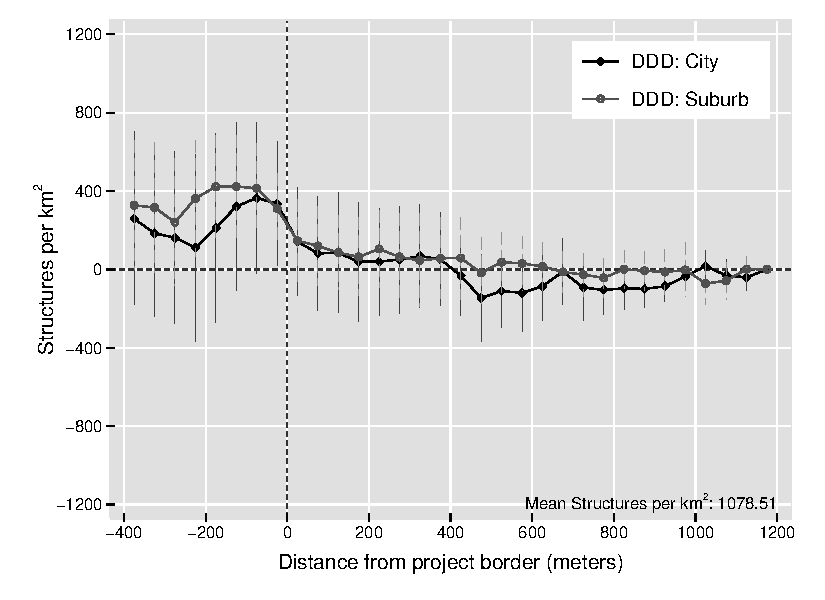
\includegraphics[width=\textwidth,trim={.5cm .3cm .3cm 0cm}, clip=true]{figures/distplotDDD_bblu_for_admin_het_2}     
        \label{fig:DDDformal_het}
    \end{subfigure}
    \vskip 1mm \vskip 0pt
    \begin{subfigure}[b]{0.49\textwidth}
        \centering
        \caption[]{\small Informal Houses}
        \vspace{-1mm}
        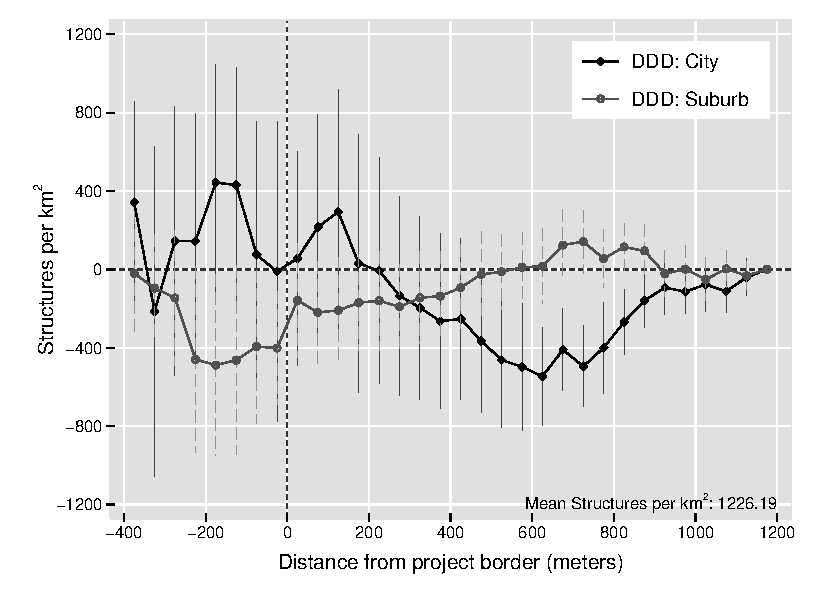
\includegraphics[width=\textwidth,trim={.5cm .3cm .3cm 0cm}, clip=true]{figures/distplotDDD_bblu_inf_admin_het_2}
        \label{fig:DDDinformal_het}
    \end{subfigure}
    \hfill
    \begin{subfigure}[b]{0.49\textwidth}  
        \centering
        \caption[]{\small Backyard Informal Houses}  
        \vspace{-1mm}
        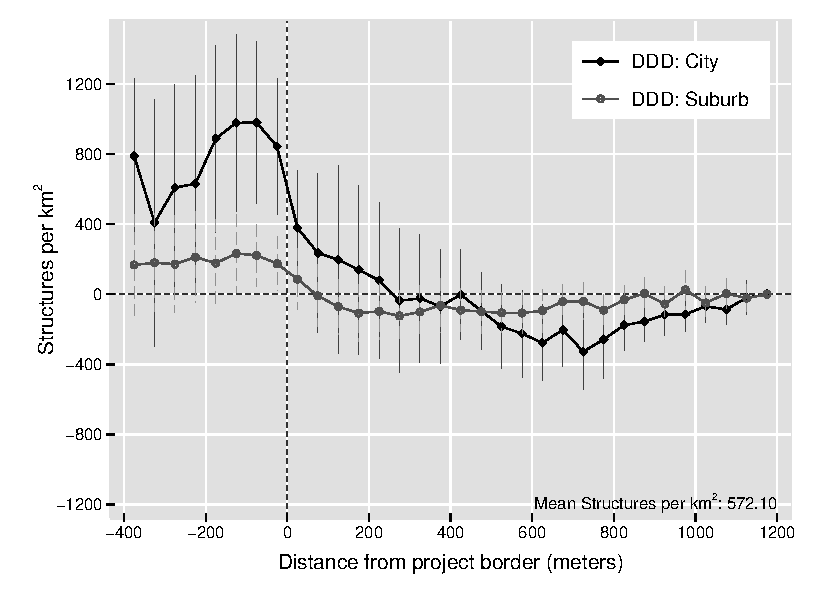
\includegraphics[width=\textwidth,trim={.5cm .3cm .3cm 0cm}, clip=true]{figures/distplotDDD_bblu_inf_backyard_admin_het_2}
        \label{fig:DDDbackyard_het}
    \end{subfigure}
    \vskip 1mm \vskip 0pt
    \begin{subfigure}[b]{.49\textwidth}  
        \centering
        \caption[]{\small Non-Backyard Informal Houses} 
        \vspace{-1mm}
        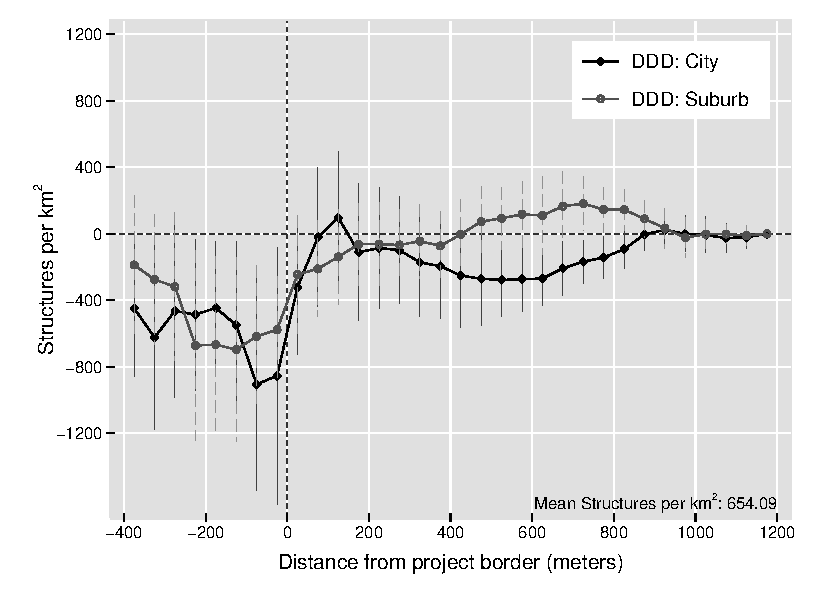
\includegraphics[width=\textwidth,trim={.5cm .3cm .3cm 0cm}, clip=true]{figures/distplotDDD_bblu_inf_non_backyard_admin_het_2}    
        \label{fig:DDDnonbackyard_het}
    \end{subfigure}
    \hfill \hspace{.02\textwidth}
    \begin{minipage}{0.47\textwidth}   
    \vspace{-6cm}
    \caption[]
    {\small DDD coefficients (equation \ref{eq:bblu}) for fives types of housing densities.} \label{fig:DDDbblu_het}
	\end{minipage}
\end{figure*} 


\begin{table}[h!]
\small
\centering
\caption{Triple Difference Estimates }\label{table:bbluDDD}
\vspace{-2mm}
\begin{tabular}{lCCCCC}
\toprule
& \small (1) & \small (2) & \small (3) & \small (4)& \small (5) \\
 & \small Total Housing & \small Formal Housing & \small Informal Housing & \small Backyard Housing & \small Non-Bkyrd Housing \\ \midrule 
-400m to 0m &      380.42\textsuperscript{c}&      383.62\textsuperscript{a}&       -3.21                   &      595.16\textsuperscript{a}&     -598.37\textsuperscript{a}\\
            &    (220.30)                   &    (137.61)                   &    (216.44)                   &    (148.74)                   &    (211.01)                   \\[0.5em]
0m to 400m  &      138.10                   &      100.48                   &       37.62                   &       97.16                   &      -59.54                   \\
            &    (140.13)                   &     (73.94)                   &    (139.85)                   &    (101.46)                   &    (103.41)                   \\ \midrule
Mean dep. var.&    2,304.71                   &    1,078.51                   &    1,226.19                   &      572.10                   &      654.09                   \\
\# Projects &         165                   &         165                   &         165                   &         165                   &         165                   \\
R$^2$       &       0.088                   &       0.115                   &       0.054                   &       0.093                   &       0.048                   \\
N           &     425,920                   &     425,920                   &     425,920                   &     425,920                   &     425,920                   \\

\bottomrule
\multicolumn{6}{l}{\footnotesize Standard errors clustered at the project level in parenthesis. \textsuperscript{c} p$<$0.10,\textsuperscript{b} p$<$0.05,\textsuperscript{a} p$<$0.01 }
\end{tabular}
\end{table}


\begin{table}[h!]
\small
\centering
\caption{Triple Difference Estimates }\label{table:bbluDDD_het}
\vspace{-2mm}
\begin{tabular}{lCCCCC}
\toprule
& \small (1) & \small (2) & \small (3) & \small (4)& \small (5) \\
 & \small Total Housing & \small Formal Housing & \small Informal Housing & \small Backyard Housing & \small Non-Bkyrd Housing \\ \midrule 
City -400m to 0m&      766.17\textsuperscript{b}&      371.37                   &      394.80                   &      981.92\textsuperscript{a}&     -587.12\textsuperscript{b}\\
            &    (301.43)                   &    (232.20)                   &    (309.44)                   &    (238.72)                   &    (282.67)                   \\
City 0m to 400m&      390.21\textsuperscript{c}&      129.14                   &      261.07                   &      226.28                   &       34.79                   \\
            &    (234.42)                   &    (117.07)                   &    (232.41)                   &    (173.78)                   &    (164.52)                   \\
Suburb -400m to 0m&      -45.17                   &      361.30\textsuperscript{b}&     -406.47                   &      231.88\textsuperscript{c}&     -638.35\textsuperscript{b}\\
            &    (226.65)                   &    (157.11)                   &    (252.88)                   &    (125.56)                   &    (311.52)                   \\
Suburb 0m to 400m&     -137.59                   &       63.20                   &     -200.79\textsuperscript{c}&      -49.05                   &     -151.74                   \\
            &    (127.99)                   &     (81.14)                   &    (117.64)                   &     (73.75)                   &    (128.53)                   \\
Mean dep. var.&    2,304.71                   &    1,078.51                   &    1,226.19                   &      572.10                   &      654.09                   \\
\# Projects City&          90                   &          90                   &          90                   &          90                   &          90                   \\
\# Projects Suburb&          90                   &          90                   &          90                   &          90                   &          90                   \\
R$^2$       &       0.126                   &       0.127                   &       0.085                   &       0.124                   &       0.055                   \\
N           &     425,920                   &     425,920                   &     425,920                   &     425,920                   &     425,920                   \\

\bottomrule
\multicolumn{6}{l}{\footnotesize ``Near'' is within 32 km from the CBD and ``Far'' is greater than 32km from the CBD.}  \\
\multicolumn{6}{l}{Standard errors clustered at the project level in parenthesis. \textsuperscript{c} p$<$0.10,\textsuperscript{b} p$<$0.05,\textsuperscript{a} p$<$0.01 }
\end{tabular}
\end{table}


\begin{figure}
\caption{Price Estimates over Distance from Project}\label{figure:distplot}
\centering
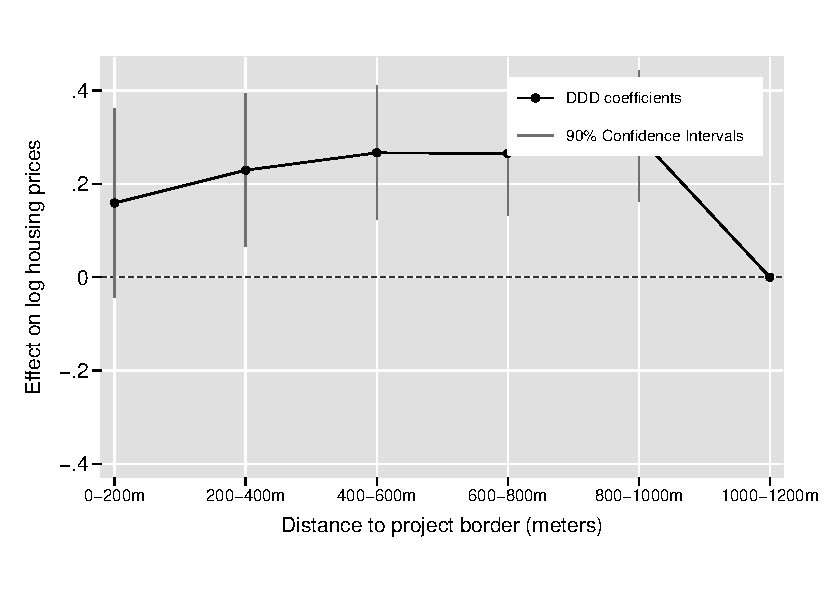
\includegraphics[width=0.9\textwidth,trim={0cm .7cm 0cm 0.7cm},clip=true]{figures/price_regs_DDDplot_2}
\vspace{-2mm}
\end{figure}

\begin{figure}
\caption{Price Estimates over Distance from Project Het}\label{figure:distplot_het}
\centering
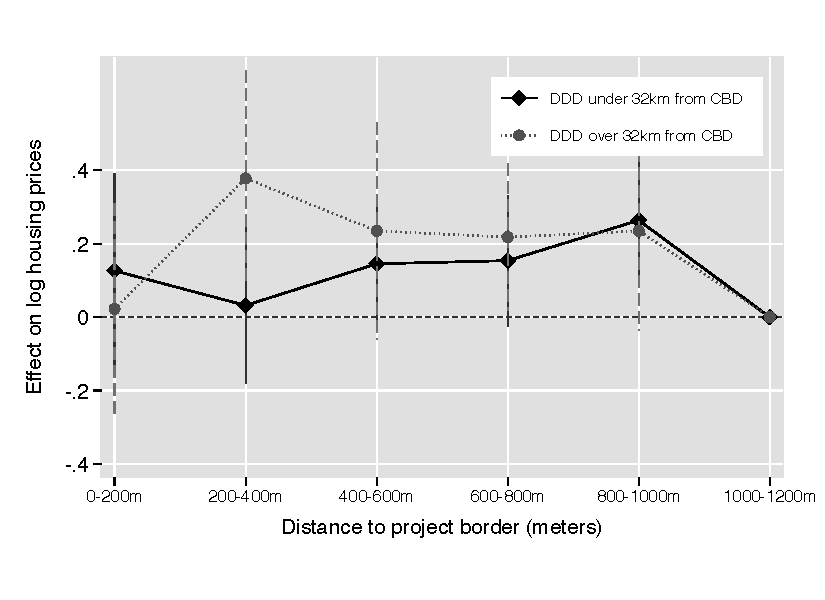
\includegraphics[width=0.9\textwidth,trim={0cm .7cm 0cm 0.7cm},clip=true]{figures/price_regs_DDDplot_het_2}
\vspace{-2mm}
\end{figure}


% \begin{table}
% \small
% \centering
% \caption{Triple Difference Estimates on Log-Prices}\label{table:priceDDD}
% \vspace{-2mm}
% \begin{tabular}{lCCCC}
% \toprule
%  & \small (1) & \small (2) & \small (3) & \small (4) \\ \midrule 
% 0 to 200m   &      -0.104&      -0.103&      -0.160&      -0.155\\
            &     (0.127)&     (0.093)&     (0.093)&     (0.118)\\[0.5em]
200m to 400m&      -0.061&      -0.058&      -0.111&      -0.104\\
            &     (0.099)&     (0.074)&     (0.084)&     (0.097)\\[0.5em]
400m to 600m&       0.057&       0.011&      -0.038&      -0.061\\
            &     (0.086)&     (0.077)&     (0.074)&     (0.073)\\ \midrule
Cubic in lot size&  \checkmark&  \checkmark&  \checkmark&  \checkmark\\
Project \textsc{FE}&           .&  \checkmark&           .&           .\\
Year{\tim}Project \textsc{FE}&           .&           .&  \checkmark&           .\\
Year{\tim}Lat-Lon cell \textsc{FE}&           .&           .&           .&  \checkmark\\
Year-Month \textsc{FE}&  \checkmark&  \checkmark&           .&           .\\
Month \textsc{FE}&           .&           .&  \checkmark&  \checkmark\\
R$^2$       &       0.174&       0.347&       0.381&       0.264\\
N           &     120,866&     120,866&     120,866&     120,866\\

% \bottomrule
% \multicolumn{5}{l}{\footnotesize Standard errors clustered at the project level in parenthesis. \textsuperscript{c} p$<$0.10,\textsuperscript{b} p$<$0.05,\textsuperscript{a} p$<$0.01 }
% \end{tabular}
% \end{table} 

% \begin{table}
% \small
% \centering
% \caption{Triple Difference Estimates on Log-Prices Het}\label{table:priceDDD_het}
% \vspace{-2mm}
% \begin{tabular}{lCCCC}
% \toprule
%  & \small (1) & \small (2) & \small (3) & \small (4) \\ \midrule 
% Near CBD 0 to 200m&      -0.067&      -0.073&      -0.059&      -0.178\\
            &     (0.198)&     (0.197)&     (0.218)&     (0.201)\\[0.5em]
Near CBD 200m to 400m&      -0.093&      -0.105&      -0.100&      -0.206\\
            &     (0.162)&     (0.119)&     (0.122)&     (0.132)\\[0.5em]
Near CBD 400m to 600m&      -0.220&      -0.228&      -0.242&      -0.291\\
            &     (0.172)&     (0.125)&     (0.131)&     (0.125)\\[0.5em]
Far from CBD 0 to 200m&      -0.538&      -0.183&       0.020&      -0.413\\
            &     (0.252)&     (0.196)&     (0.223)&     (0.292)\\[0.5em]
Far from CBD 200m to 400m&      -0.179&       0.188&       0.306&       0.019\\
            &     (0.251)&     (0.191)&     (0.195)&     (0.130)\\[0.5em]
Far from CBD 400m to 600m&      -0.162&       0.248&       0.358&       0.043\\
            &     (0.264)&     (0.272)&     (0.250)&     (0.297)\\
Cubic in lot size&  \checkmark&  \checkmark&  \checkmark&  \checkmark\\
Project \textsc{FE}&           .&  \checkmark&           .&           .\\
Year{\tim}Project \textsc{FE}&           .&           .&  \checkmark&           .\\
Year{\tim}Lat-Lon cell \textsc{FE}&           .&           .&           .&  \checkmark\\
Year-Month \textsc{FE}&  \checkmark&  \checkmark&           .&           .\\
Month \textsc{FE}&           .&           .&  \checkmark&  \checkmark\\
R$^2$       &       0.202&       0.334&       0.356&       0.289\\
N           &      87,253&      87,253&      87,253&      87,253\\

% \bottomrule
% \multicolumn{5}{l}{\footnotesize Standard errors clustered at the project level in parenthesis. \textsuperscript{c} p$<$0.10,\textsuperscript{b} p$<$0.05,\textsuperscript{a} p$<$0.01 }
% \end{tabular}
% \end{table} 

% \begin{figure}[t!]
% \caption{Time-to-Event Price Estimates}\label{figure:timeplot}
% \centering
% 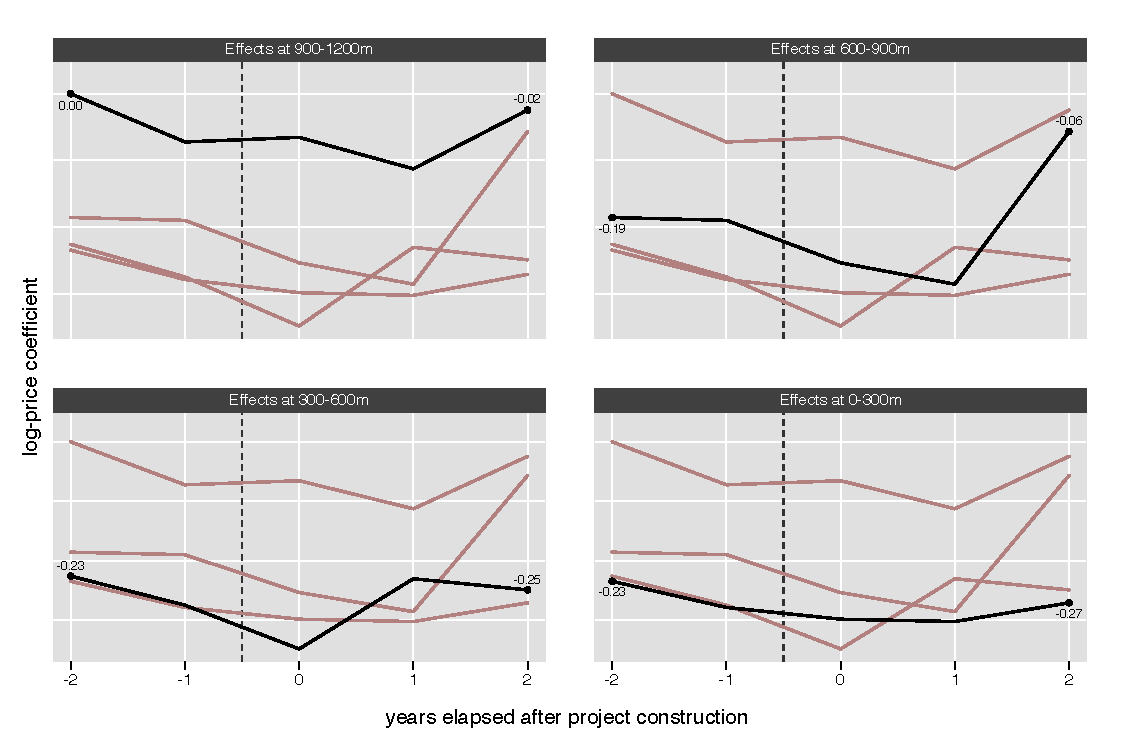
\includegraphics[width=0.99\textwidth,trim={0cm 0cm 0cm 0cm},clip=true]{figures/DDDplot_pertime_alt_unspaghetti}
% \vspace{-2mm}
% \end{figure}




\end{document}


